%%%%%%%%%%%%%%%%%%%%%%%%%%%%%%%%%%%%%%%%%%%%%%%%%%%%%%%%%%%%%%%%%%%%%%%%%%%%%%%%

% IEEEconf.cls file must exist in the same directory as the TeX file you want to compile
\documentclass[letterpaper, 10 pt, conference]{IEEEconf}

\title{\LARGE \bf
COMPUTER GAME HISTORY\\
\large The Creation and Advancements of Video Games
}

\author{Group 7\\
\small Miguel Martinez\\
\small Jeremiah Davis\\
\small Tyler Pennebaker\\
}

% Image/graphics support
\usepackage{graphicx}
\graphicspath{ {./images/} }

% Formatting for lists
\usepackage{enumitem}

% Formatting for media
\usepackage{float}
\restylefloat{table}
\restylefloat{figure}

\begin{document}


\maketitle
\thispagestyle{empty}
\pagestyle{empty}


%%%%%%%%%%%%%%%%%%%%%%%%%%%%%%%%%%%%%%%%%%%%%%%%%%%%%%%%%%%%%%%%%%%%%%%%%%%%%%%%
\section*{ABSTRACT}
\textit{
Video games are a form of entertainment which includes interaction with a user interface. The interaction is dependant on images produced by a computer program. Since the birth of video games, they advance and evolve at a rapid rate.
}

%%%%%%%%%%%%%%%%%%%%%%%%%%%%%%%%%%%%%%%%%%%%%%%%%%%%%%%%%%%%%%%%%%%%%%%%%%%%%%%%
\section{INTRODUCTION}

With a starting development in the 1960's, video games have had plenty of advancements and have grown to extremely monetizable around the world. We chose to research this topic because we are all familiar with, and enjoy video games. The creation of computer programs intended for video games is an interesting process and the growth of computer programming and its impact on the world today is astonishing.

%%%%%%%%%%%%%%%%%%%%%%%%%%%%%%%%%%%%%%%%%%%%%%%%%%%%%%%%%%%%%%%%%%%%%%%%%%%%%%%%
\section{TIME PERIOD}

The invention of video games began in the 1960's. Advancements in computers convenience and interactivity encouraged peoples curiosity with computers and software. Video games initial use were not monetization, they were simply made for the creators own entertainment and curiosity. The creation and monetization of one of the earliest games known as Pong sprouted the video game industry and led it to be one of the most profitable and marketable industry's today.

%%%%%%%%%%%%%%%%%%%%%%%%%%%%%%%%%%%%%%%%%%%%%%%%%%%%%%%%%%%%%%%%%%%%%%%%%%%%%%%%
\section{COMPUTER HARDWARE}

The hardware used early on was simple though at the time it was considered revolutionary. The first commercially successful game console was the Magnavox Odyssey which ran games such as table tennis and Analogic. The Magnavox Odyssey two, their second console, was an 8-bit console, its RAM was only capable of 64 bytes, and a resolution output of 280x192, all of which are vastly outdated when compared to today's standards. Now the Magnavox Odyssey is out of the market, however new consoles have taken its place. Game consoles and Commuters are now able to put much more power into games, meaning instead of games like pong, we get games with ultra realistic graphics, higher resolutions, and better performance than could have ever been dreamed.
\ref{tbl:example} for an example of a table.



\begin{table}[h!]
\begin{center}
\begin{tabular}{||c | c | c | c||} 
\hline
  & RAM & Bits & Resolution \\ [0.5ex]
\hline\hline
Magnavox Odyssey 2 & 64 Bytes & 8 & 280x192 \\ 
\hline
PS5 & 16GB GDDR6 & 64 & 4K \\
\hline
Xbox series X & 16GB GDDR6 & 64 & 4K \\
\hline
\end{tabular}
\caption{Spec comparison of first consoles to modern ones }
\label{tbl:example}
\end{center}
\end{table}

\begin{figure}[h!]
\centering
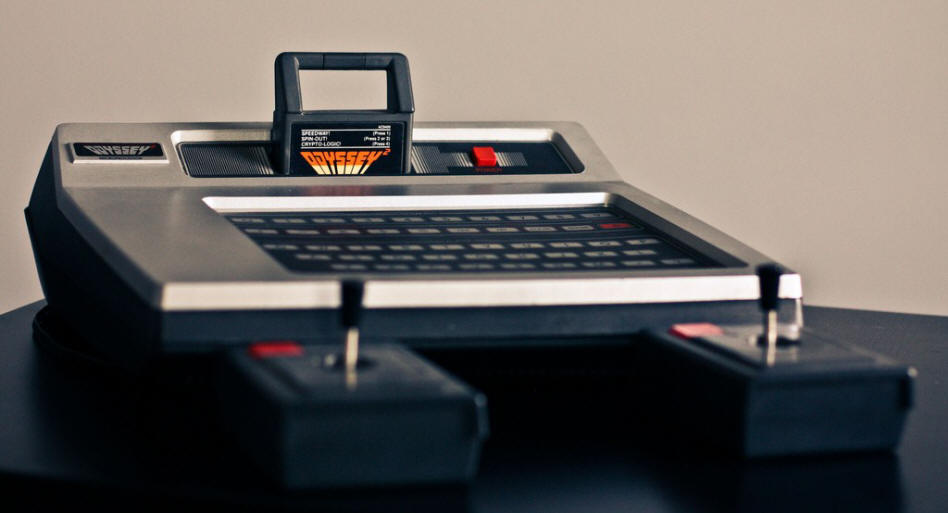
\includegraphics[width=0.5\textwidth]{images/odyssey2-front.jpg}
\caption{Magnavox Odyssey 2}
\label{fig:example}
\end{figure} 

\section{COMPUTER SOFTWARE}

Describe the software used for your chosen topic if any,
and state any uses of the software that your topic had.
If your topic does not have or use software, describe why it
doesn't use software and how it functions without it.

\section{CONCLUSION}

Conclude your research paper with any reflections on what you
learned about your topic. Was this what you expected to find?
Did you find any facts that surprised you? You may add other
personal reflections about the topic here.

\section*{REFERENCES}

Below are basic formats for different types of references.

\begin{enumerate}[label={[\arabic*]}]
\item Name of Author, ``Title of chapter in the book,''
Title of The Published Book, xth edition. City of
Publisher, Country if not U.S.
\item Name of Author, “Name of paper,” Abbrev.
Title of Periodical, vol. x, no. x, pp. xxx-xxx,
Abbrev. Month, year.
\item Name of Author, (Year, Month),
Title of Internet Article [Online]. Available E-Mail:
E-Mail.
\end{enumerate}

\end{document}

